\begin{figure}[!t]
  \centering
  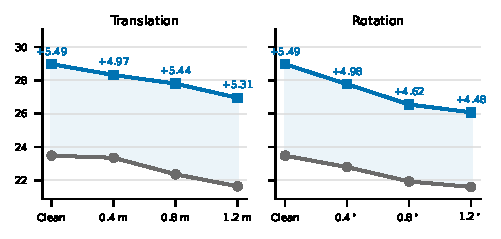
\includegraphics[width=\columnwidth]{figures/fig12-robustness-curves.pdf}
  \caption{\textbf{Robustness difference between \nameplus{} (C) and Plain (C).}
  The two panels report absolute dynamic mIoU under translation and rotation
  re-anchoring. Gray circles denote Plain (C), blue squares denote
  \nameplus{} (C), and the numbers above each setting denote
  \nameplus{} (C) minus Plain (C).}
  \label{fig:robustness_c_prosd_vs_plain}
\end{figure}
